%!TEX program = xelatex
% 完整编译: xelatex -> bibtex -> xelatex -> xelatex
\documentclass[lang=cn,11pt,a4paper,cite=authoryear]{elegantpaper}

\title{基于聚类与时间序列的H指数增长预测分析}
\author{李子岳 \\ 经71  \and 肖昌荣 \\ 经71}
\institute{清华大学经济管理学院}

%\version{0.09}
\date{\zhtoday}


% 本文档命令
\usepackage{array}
\newcommand{\ccr}[1]{\makecell{{\color{#1}\rule{1cm}{1cm}}}}
\usepackage{booktabs}
\usepackage{float}

\begin{document}

\maketitle

\begin{abstract}
H指数是目前学界公认的一种衡量学者学术影响力和科研成果的重要指标,如何对H指数的增长进行预测,进而评价学者未来的学术影响力便得到许多研究者的关注。本文将使用计算机科学领域知名学者的数据集,对数据进行聚类分析来比较不同类别学者的异同,从中发现不同类别的学者有类内统一的指数增长、线性增长两种H指数增长模式。我们进一步利用聚类得到的启示,构建一种基于聚类的H指数预测模型,从现有数据中充分提取信息辅助预测。由于聚类启发式模型具有一定的局限性,我们接着提出适用范围更广的基于时间序列的ARIMA模型,并验证了该模型在数据集中有较为准确且稳健的预测效果,综合来说是相当优秀的模型。最后,我们总结了所提出的两种模型的优缺点,讨论H指数这一指标对于衡量一位学者的学术水平是否合理、有效,并归纳之前学者对指标的补充完善,提出对于预测学者学术影响力的更多思路。
\keywords{H指数,预测,时间序列,聚类}
\end{abstract}

\section{导言}

\subsection{H指数简介}

H指数由\cite{Hirsch16569}在2005年提出,目的是量化学者的影响力和科研成果,对他们进行评估与比较。假设一位学者在n年内发表的论文数为$N_p$,每篇论文的被引数为$N_c^j$,则这个学者的“H指数=$h$”表示,在他的所有论文中,至少有$h$篇论文满足,每篇论文至少被$h$篇论文引用;而对于其他($N_p-h$)篇论文,每篇的引用量小于等于$h$。\cite{Hirsch16569}的论文找出了H指数与总引用数$N_{c,tot}$之间近似满足$N_{c,tot}=ah^2$;同时发现从引用数最多到引用数最少排序的情况下第$y$篇论文的引用数$N_c (y)$与$h$和其他指标的关系,并从理论上和经验上确定了相关参数的取值范围。

\subsection{H指数的预测}

自从\cite{Hirsch16569}提出H指数的概念之后,H指数逐渐被学界接受为一种衡量学者学术能力的重要指标。正因为H指数对于衡量学术影响力的重要性,许多学者已经尝试预测不同领域学者的H指数增长趋势,进而预测其学术影响力的变化。

\cite{7397965}提出了一种基于回归的预测方法,作者使用计算机科学领域的数据集最终拟合出的最优模型使用了当前的H指数值、发表的文章数量、总引用量、合作者的数量以及从第一篇文章发表至今的年数作为回归自变量,最终预测近5年的H指数得到了很不错的结果,但对于更久远的预测以及H指数较高的学者的预测就不够准确。鉴于他们的成功,本文所收集的学者数据也属于计算机科学领域,数据集中包含了该篇文章中使用的回归因子。然而我们在构建模型时发现,按照我们收集的数据拟合后,最优的自回归参数p并不是1,且其他回归因子的效果也不是很好,但我们认为这些回归因子仍然存储着一些能辅助预测的信息,于是尝试使用聚类的方法提取数据中的相关信息,我们将在后文第4部分的ARIMA模型构建中详细介绍。

\cite{PennerPan-511}的研究则强调了“学术年龄”,也就是从第一篇文章发表至今的年数的重要性。因为H指数是一个随着时间积累的数,与学术年龄有很强的相关性。于是我们将H指数的历史数据看作时间序列,使用时间序列分析的方法构建整合移动平均自回归模型(ARIMA模型)来进行预测。同时,作者们认为在预测时需要消除H指数随时间积累的性质,即进行差分,这与我们所考虑的ARIMA模型恰好吻合。

本文所提出的两个模型正是基于\cite{7397965}与\cite{PennerPan-511}的研究,强调学术年龄的重要性,发现回归模型应用于本文数据集的不合理之处,尝试从回归模型中提取有用信息,最终总结出简洁高效的时间序列模型。

\subsection{内容梳理}

本文将使用搜集到的计算机科学领域知名学者的数据集,在第2部分对数据进行聚类分析,比较不同类别学者的异同,发现不同类别的学者有指数增长、线性增长两种H指数增长模式,且类内学者的增长模式基本统一。第3和第4部分分别为我们提出的两种H指数增长预测模型,其中在第3部分利用聚类得到的启示,构建一种基于聚类的H指数预测模型,尽可能多地从现有数据中提取信息辅助预测。由于聚类启发式模型的局限性,我们进一步在第4部分提出适用范围更广的基于时间序列的ARIMA模型,验证了该模型在数据集中有较为准确且稳健的预测效果,综合来说是相当优秀的模型。最后,我们在第5部分总结了所提出的两种模型的优缺点,进一步讨论H指数这一指标对于衡量一位学者的学术水平是否合理、有效,并归纳了之前学者对H指数的补充完善。


\section{数据集简介与分析}

\cite{Bar-Ilan2008}讨论了收集H指数的主要数据来源,分别是Scopus、Web of Science和Google Scholar。其中,前两种是知名数据库,各大高校图书馆均已订购,可以获取历年引文数据;而Google Scholar是公开的数据。\cite{Bar-Ilan2008}提到,Google Scholar会高估H指数,而他使用了Web of Science的数据。我们在此使用Scopus的数据,因为Scopus能够快速、准确、方便定位学者,并且提供了更多丰富的信息。我们从Scopus中收集了96 个计算机科学领域的知名学者的数据,之所以只收集学术影响力高的知名学者的数据,是因为普通学者的H指数往往偏低,且随时间的变化不大,研究他们的H指数增长规律意义较小。而这些知名学者,则是从\url{http://www.guide2research.com/scientists/}的信息中抽取的。而这些学者在Scopus中检索的结果表明其H指数相对较高,所以这也证明了数据来源的可靠性。

数据集的详细介绍如表(\ref{tab1})所示:

\begin{table}[H]
	\centering
	\caption{数据集内容简介}
	\label{tab1}
	\begin{tabular}{@{}llp{8cm}@{}}
		\toprule
		\multicolumn{1}{c}{名称} & \multicolumn{1}{c}{数据类型} & \multicolumn{1}{c}{解释}                          \\ \midrule
		\textit{h-index}                & 列表                       & 从1970年至2020年该学者截止每年的h指数值。若在某年份之前该学者还未发表文章,则标为0。 \\
		\textit{earliest\_year}         & 整数值                      & 该学者发表最早一篇文章的年份。                                 \\
		\textit{academic\_age}          & 整数值                      & 该学者从发表最早一篇文章的年份至今(2020年)的年数,称为“学术年龄”。           \\
		\textit{co-author}              & 整数值                      & 该学者截止2020年的合作者数。                                \\
		\textit{paper\_num}             & 整数值                      & 该学者截止2020年发表的文章数。                               \\
		\textit{citation\_num}          & 整数值                      & 该学者截止2020年的总被引用量。                               \\
		\textit{journal\_num}           & 整数值                      & 该学者截止2020年的所有发表文章所在期刊数。                         \\ \bottomrule
	\end{tabular}
\end{table}

其中数据集中所有学者截止2020年的H指数值的分布从25至131,发表的文章总数从112篇至1409篇,总被引用量从3697次到138785次,发表最早一篇文章的年份从1941年至2002年,于是学术年龄的范围就为18年至79年。

\subsection{聚类分析}

为了更清晰地发现数据的特点,我们以截止2020年的H指数值、学术年龄、发表文章数量、总引用量为学者数据的特征,对学者进行聚类分析。之所以没有加入合作者总数、发表的不同期刊数,是因为在去除异常值后二者与发表文章数有较为明显的线性相关关系。聚类使用\textit{K-Means}方法,Python代码调用\textit{sklearn.cluster.KMeans}实现。在对数据进行标准化后,我们计算对于指定范围内不同聚类类别数\textit{k}值所对应的误差平方和(\textit{Sum of the Squared Errors, SSE}),画出图(\ref{fig1}),使用“手肘法”观察得到\textit{k}的最佳取值为4。

\begin{figure}[H]
	\centering
	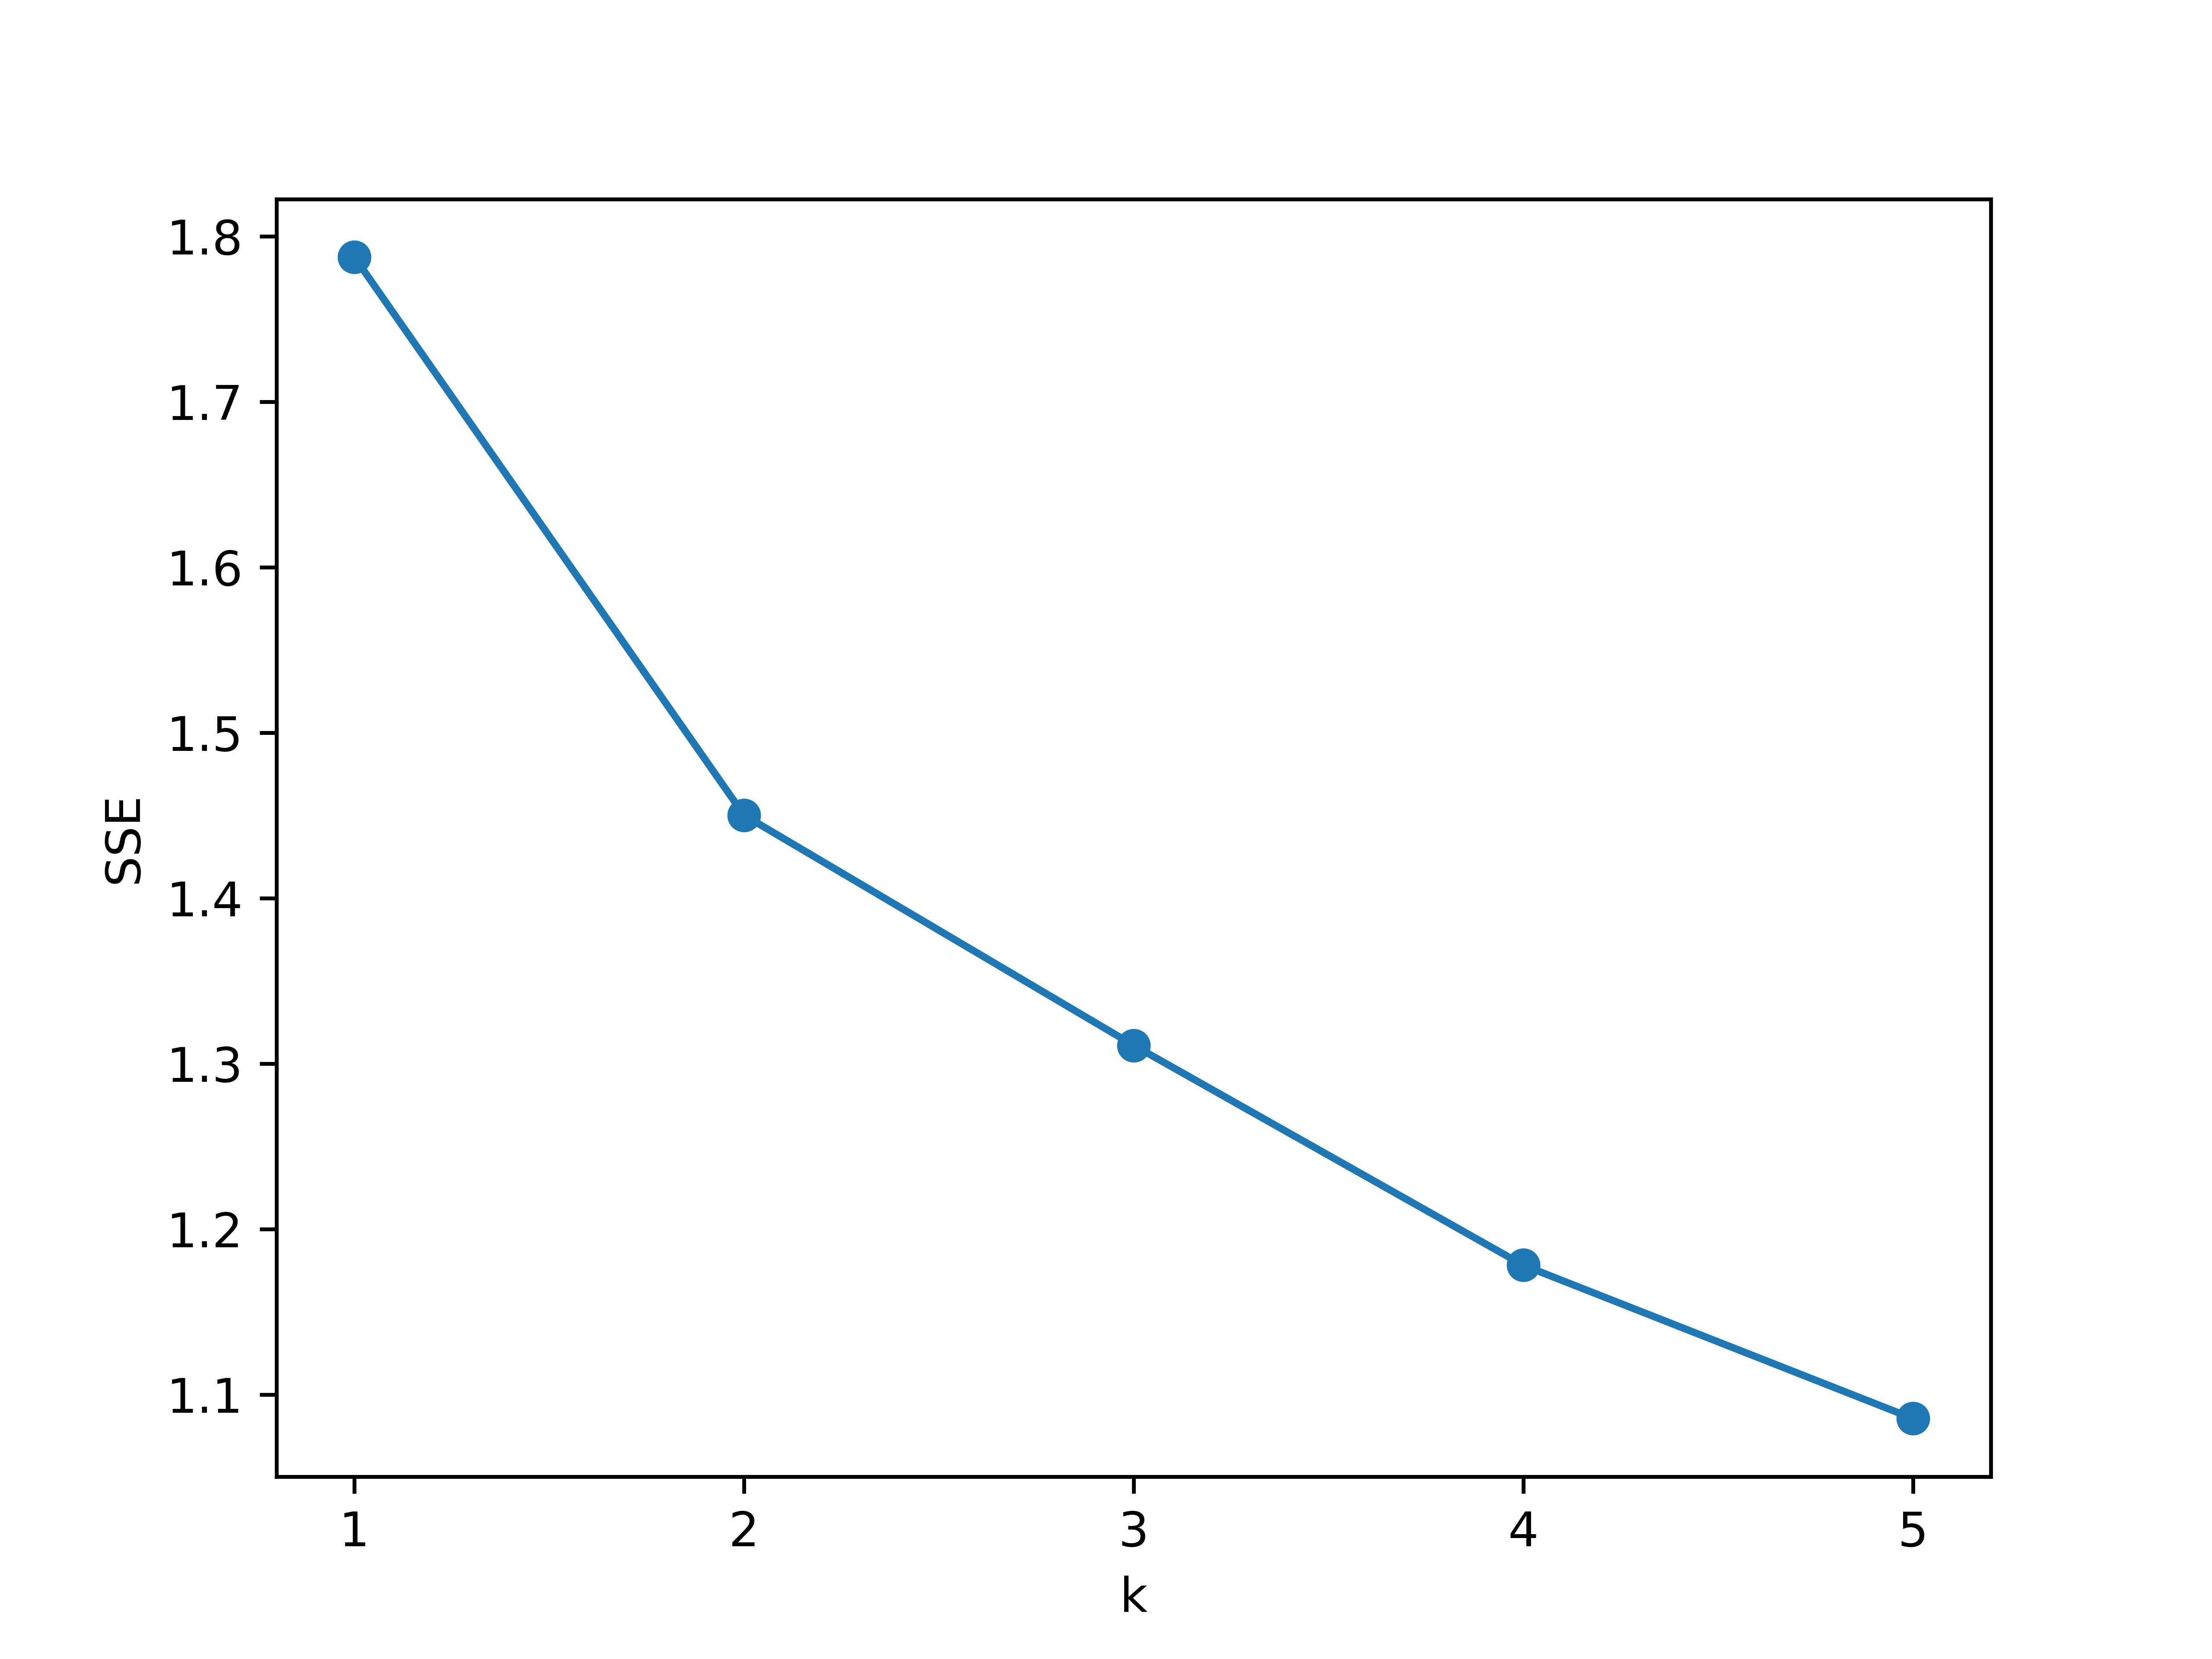
\includegraphics[width=0.6\textwidth]{image/elb.png}
	\caption{“手肘法”误差平方和图像}
	\label{fig1}
\end{figure}

当\textit{k}取4时,\textit{KMeans}方法聚类得到的结果如图(\ref{fig2})所示。其中不同颜色代表不同的类别,点的大小代表该学者H指数的大小。

\begin{figure}[H]
	\centering
	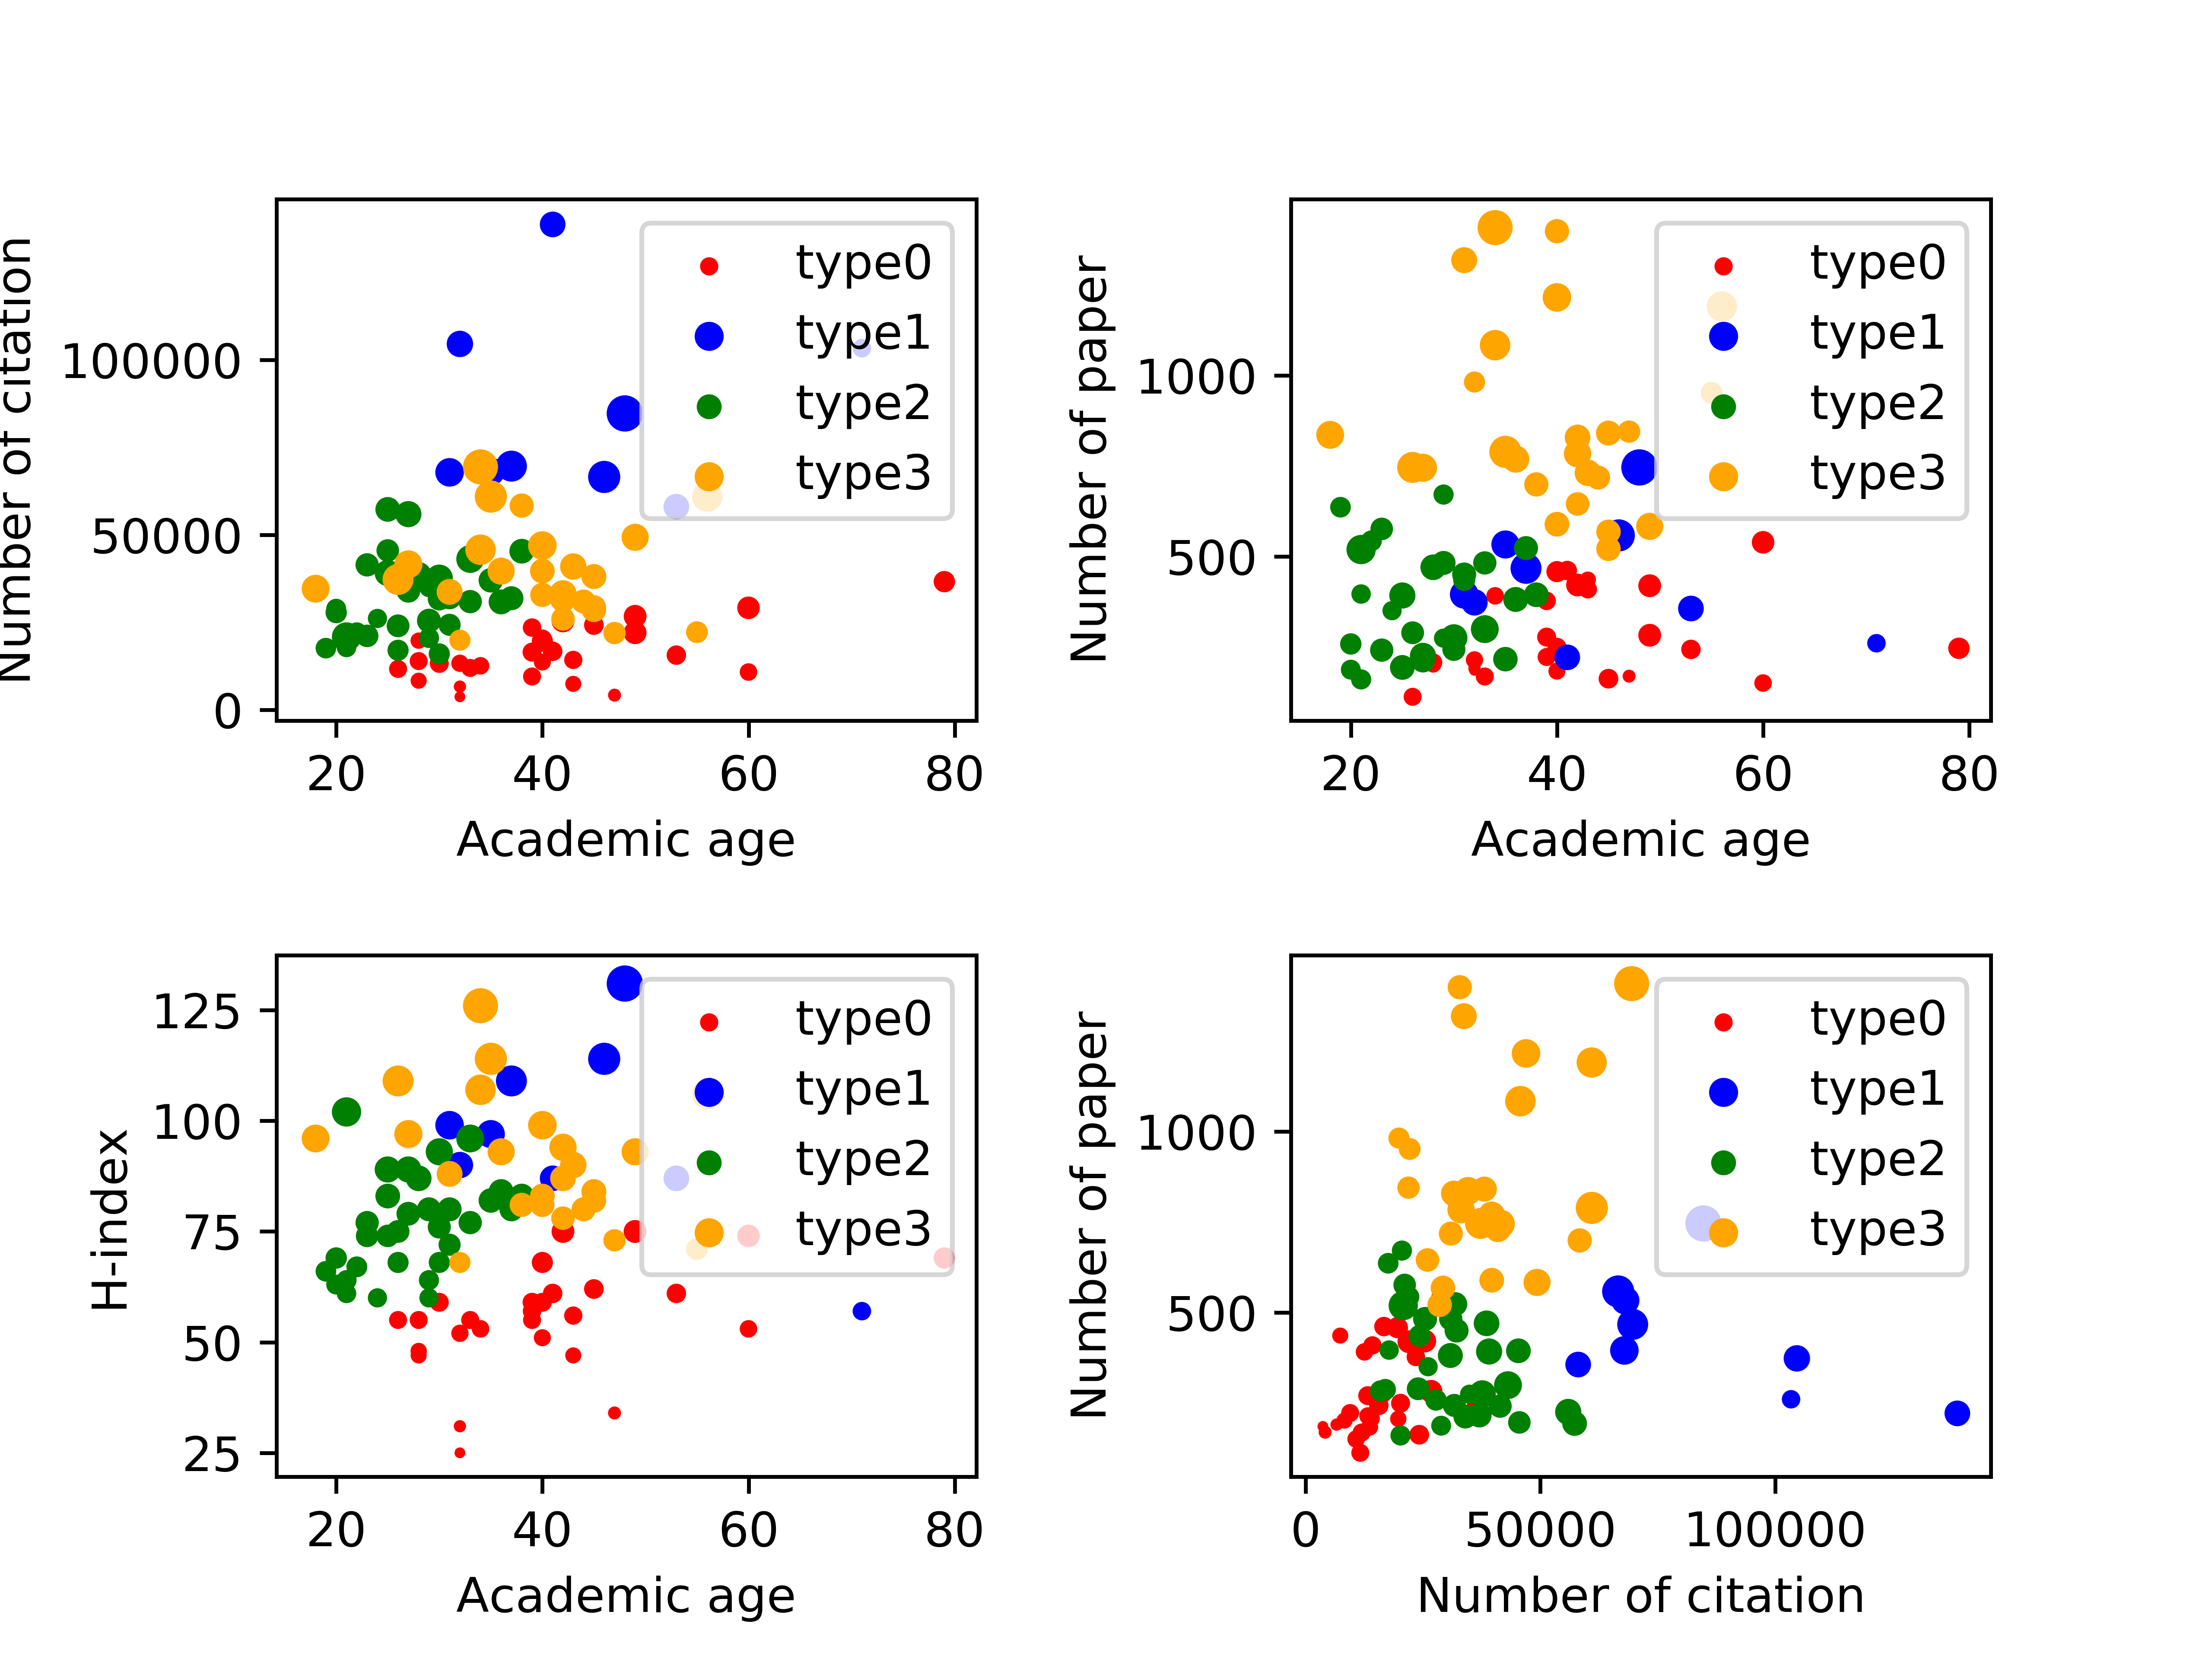
\includegraphics[width=0.9\textwidth]{image/cluster_figure.png}
	\caption{聚类结果散点图}
	\label{fig2}
\end{figure}

从上图能够清晰地观察到四个类别的特点,为了简洁直观,我们将红色的\textit{type0}称为\textbf{较弱势学者},蓝色的\textit{type1}称为\textbf{引用量优势学者},绿色的\textit{type2}称为\textbf{年轻型学者},黄色的\textit{type3}称为\textbf{文章量优势学者},他们的具体特点总结如下:

\begin{itemize}
	\item \textbf{较弱势学者}:这类学者分布于各个学术年龄段,无论是发表文章数、总引用量,还是H指数都属于四个类别学者中最低的一个。需要说明的是,该数据集中的学者都属于知名学者,较弱势类学者的绝对水平并不低,只是相对于该数据集中的其他知名学者显得处于弱势而已。一个可能的原因是该类学者的研究方向不属于热门,因而H指数值并不突出;也有可能是一些中国学者,文章较多在国内期刊发布,而较少在国外期刊发布,故一部分文章和引用量没有统计上。
	\item \textbf{年轻型学者}:这类学者的学术年龄相对而言是最年轻的,发表文章数、总引用量、H指数值中等,有较大的发展潜力。
	\item \textbf{引用量优势学者}:这类学者虽然发表文章数不多,但总引用量是最高的,进而H指数值也普遍很高。他们的学术年龄分布在30至50年之间,是以文章质量为优势的资深学者。
	\item \textbf{文章量优势学者}:这类学者与引用量优势学者相反,他们的总引用量不是最高,但凭借高发表文章数得到较大的H指数。他们的总体学术年龄比引用量优势学者低,其中部分学者以很低的学术年龄获得了超高发表文章数和不错的引用量,算是学术界的“年轻”人才。
\end{itemize}

\subsection{H指数增长规律分析}

在这一部分,我们将对上文聚类得出的四个类别及其中的一些典型学者,分析他们H指数曲线的变化规律。

首先我们查看托马斯·凯拉斯(Thomas Kailath)的H指数增长曲线,如图(\ref{fig3})。凯拉斯是斯坦福大学的电气工程师、信息理论家、控制工程师、企业家,也是日立美国工程学教授,他的著作《线性系统》被列为线性系统领域参考最多的书之一。他在聚类时被分为\textbf{较弱势学者},也许是因为他所研究的领域相比起其他计算机科学的领域较为冷门,这也验证了我们之前对于较弱势学者的一个猜测。同时,通过观察他和所有较弱势学者的H指数增长趋势,我们发现较弱势学者的H指数增长较为缓慢,更适合用\textbf{线性模型}进行拟合。

\begin{figure}[H]
	\centering
	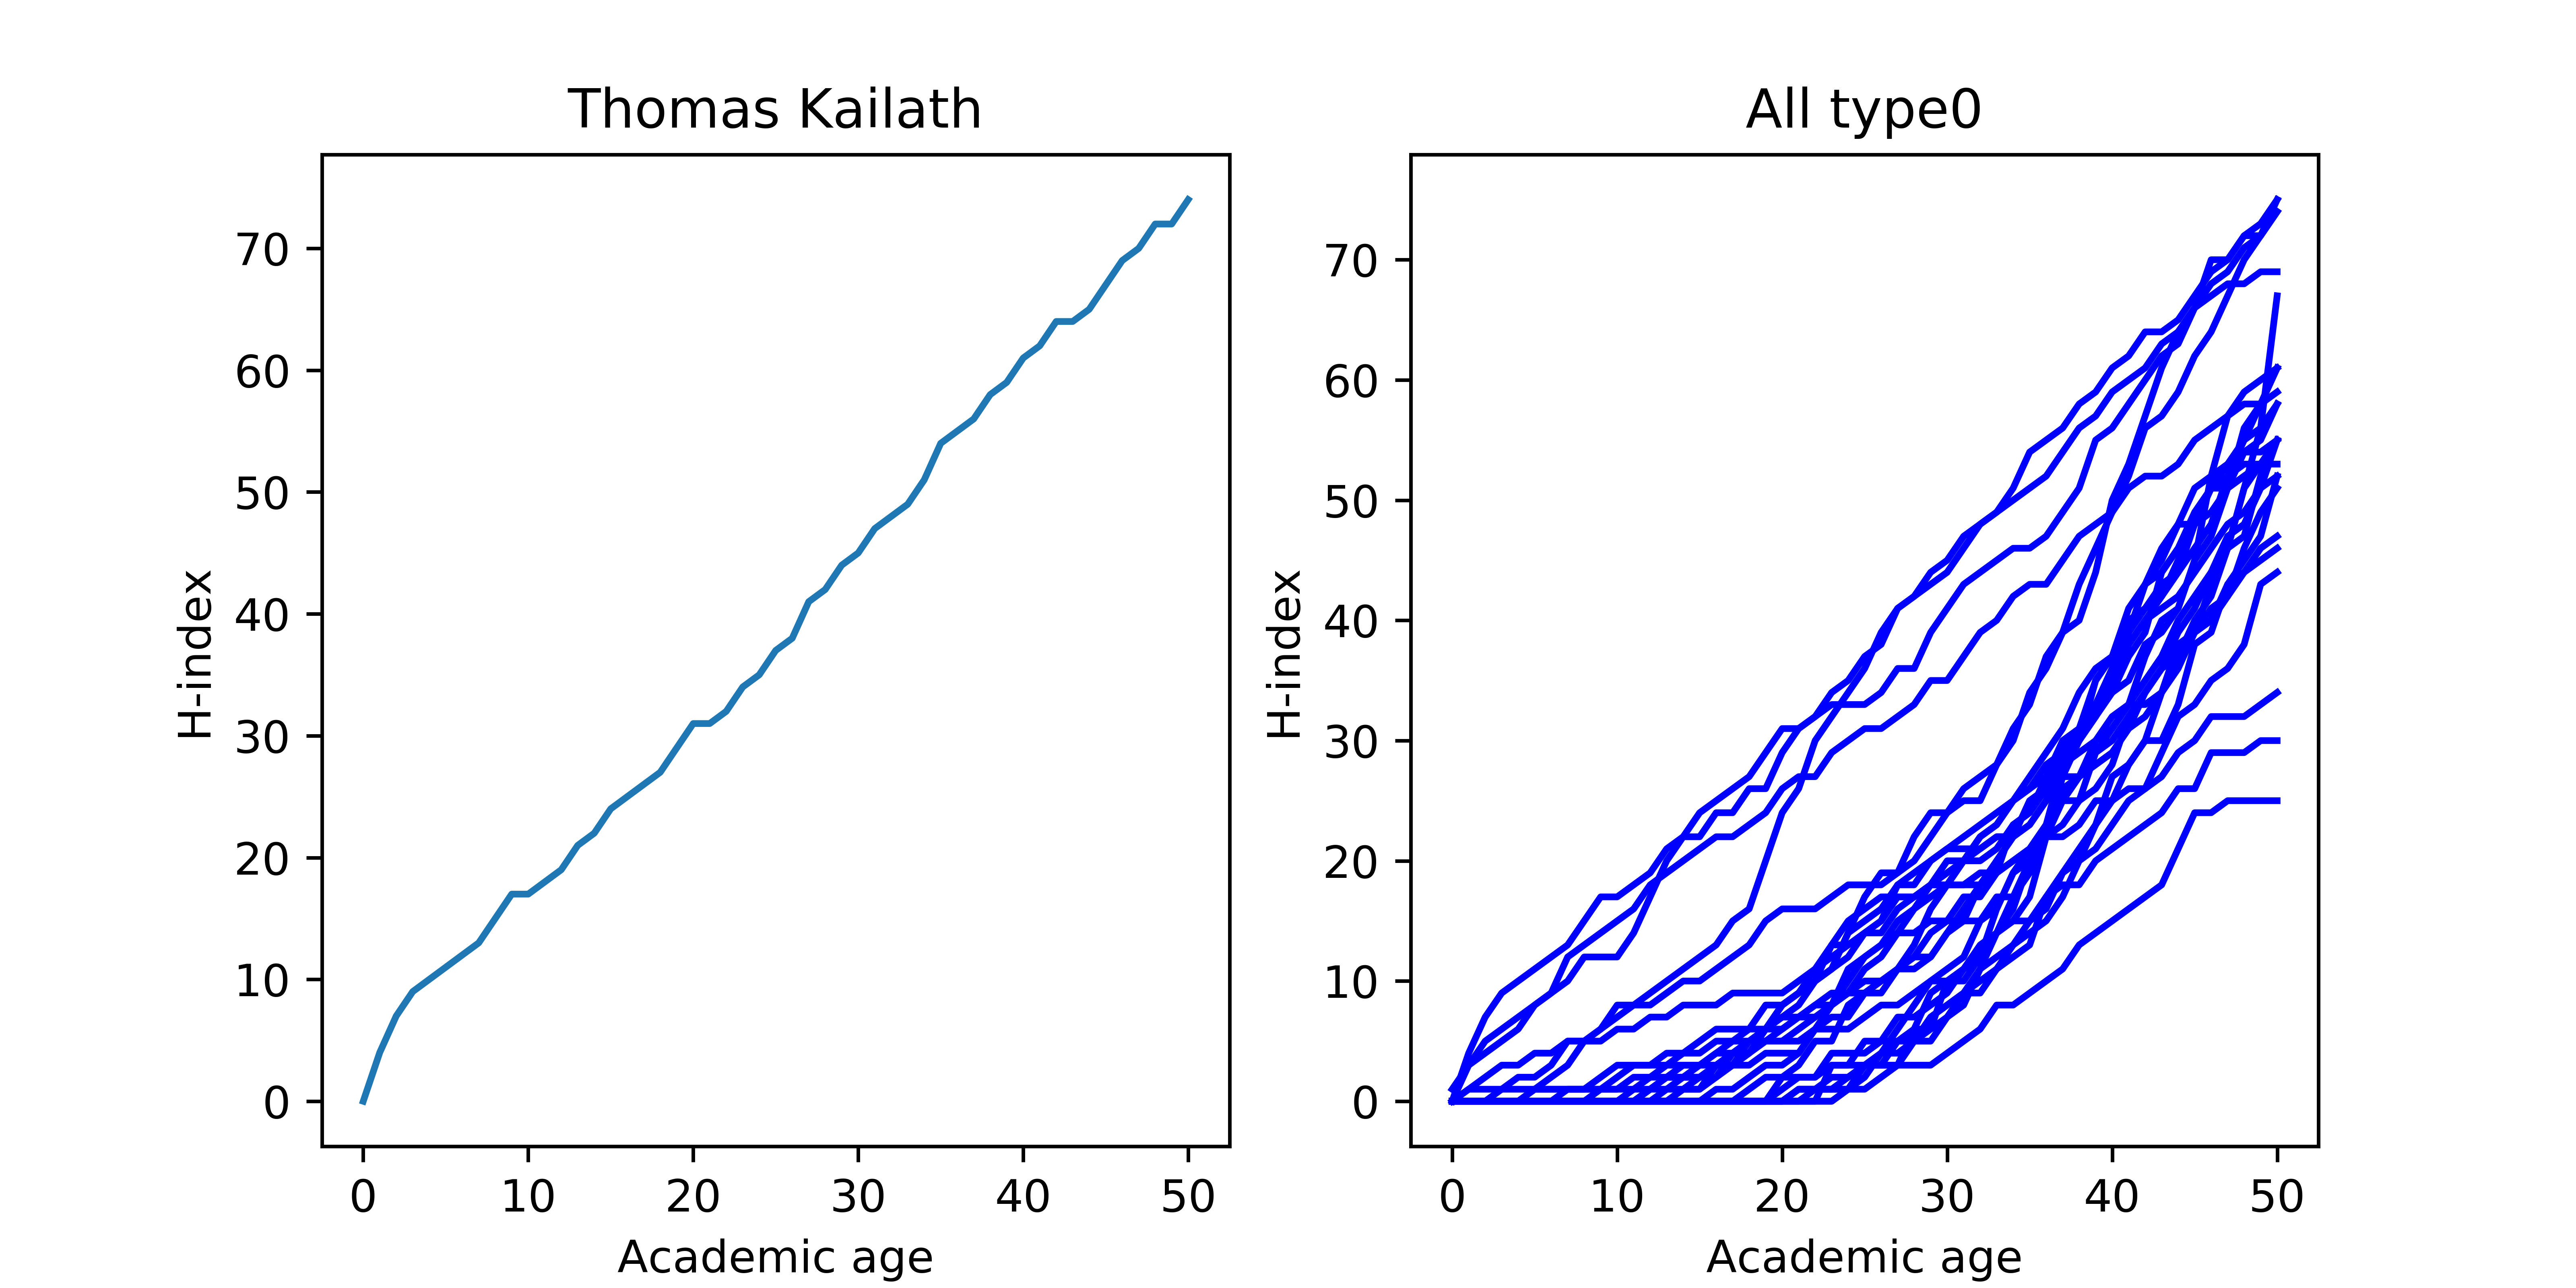
\includegraphics[width=0.9\textwidth]{image/Thomas Kailath.png}
	\caption{Thomas Kailath及较弱势学者的H指数增长曲线}
	\label{fig3}
\end{figure}

接着查看约书亚·本希奥(Yoshua Bengio)的H指数增长曲线,如图(\ref{fig4})。他属于\textbf{引用量优势学者},是人工神经网络和深度学习领域公认的著名学者,他的H指数增长曲线近似\textbf{指数函数},同样的,所有引用量优势学者中除了一位异常,他们的增长曲线都可以看做指数函数。与他一同获得2018年图灵奖的学者Geoffrey Hinton也被分为引用量优势学者,一定程度上映证了聚类的合理性。

\begin{figure}[H]
	\centering
	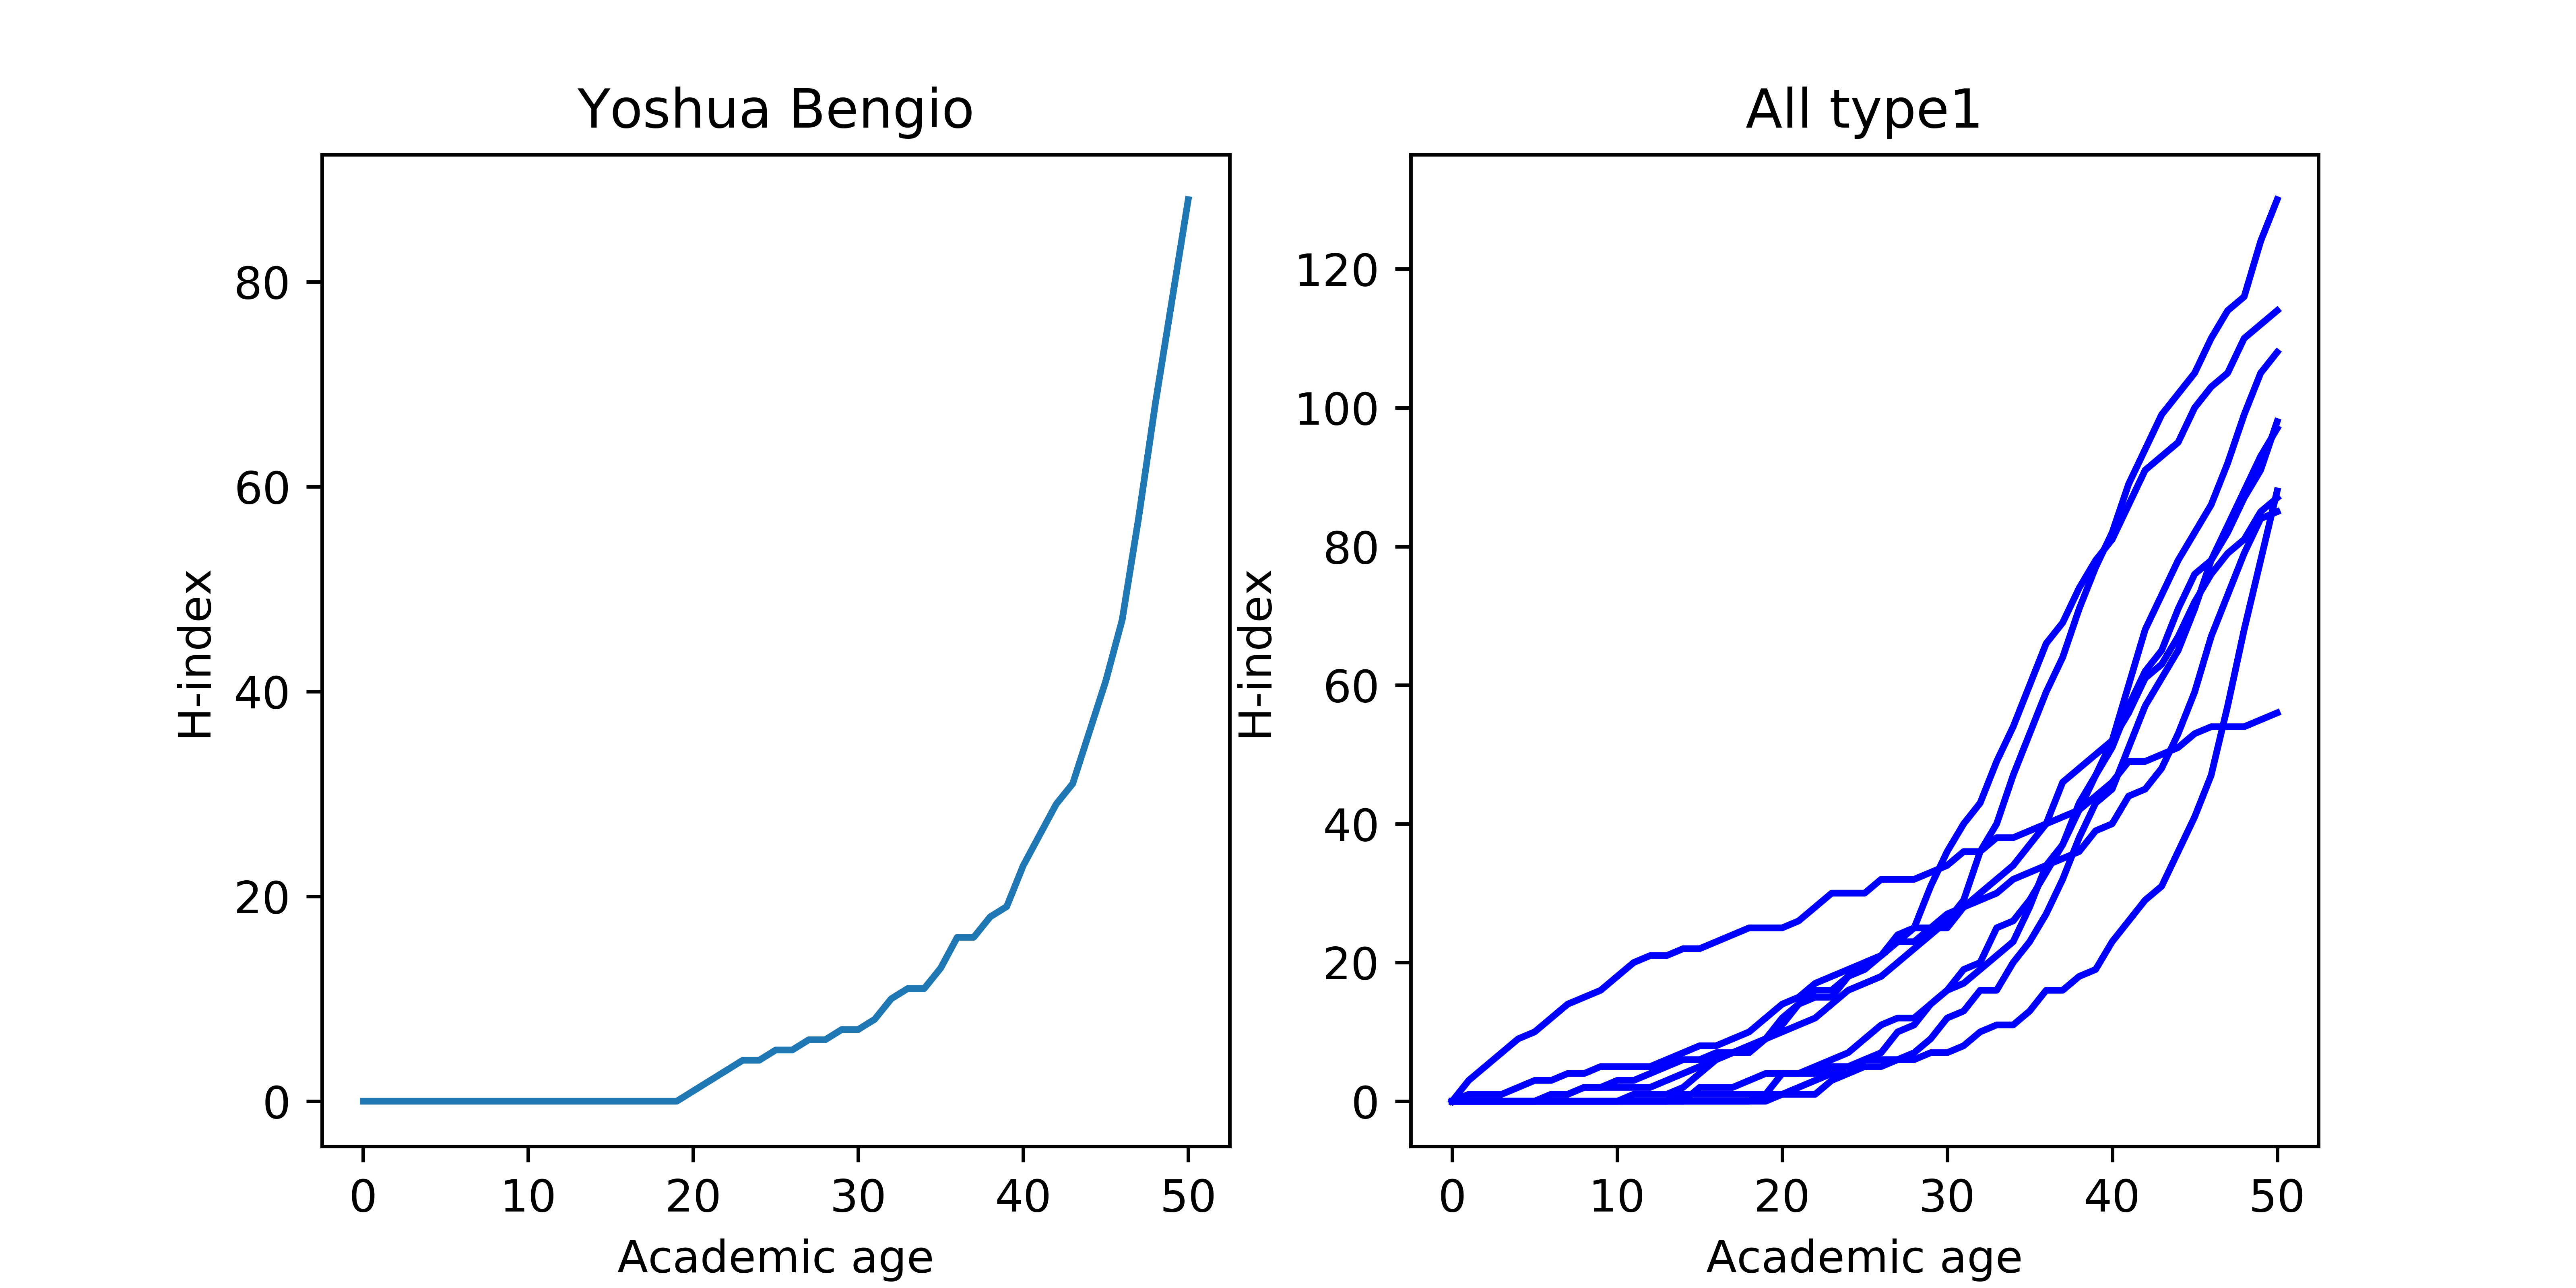
\includegraphics[width=0.9\textwidth]{image/Yoshua Bengio.png}
	\caption{Yoshua Bengio及引用量优势学者的H指数增长曲线}
	\label{fig4}
\end{figure}

对于\textbf{年轻型学者}和\textbf{文章量优势学者},他们整体的H指数变化趋势都呈\textbf{指数增长}(见图(\ref{fig5})),一些学者在最后几年的增长速度略有下降,有轻微的S型趋势。而年轻型学者的增长速率整体要高于引用量优势学者和文章量优势学者,这是因为我们所收集的数据都是有影响力的知名学者,学术年龄相对较低的学者想要与相对资深的学者比肩,必然需要有更高的H指数增长率。即数据集中的年轻型学者都“年轻有为”,H指数较低的年轻学者数据并没有被收集。而这不意味着没有出现在数据集中的年轻学者日后没有机会成为优秀的知名学者,因为数据表明一些资深的优秀学者在年轻时H指数的增长曲线也较为平缓,如数据集中的较弱势学者。

\begin{figure}[H]
	\centering
	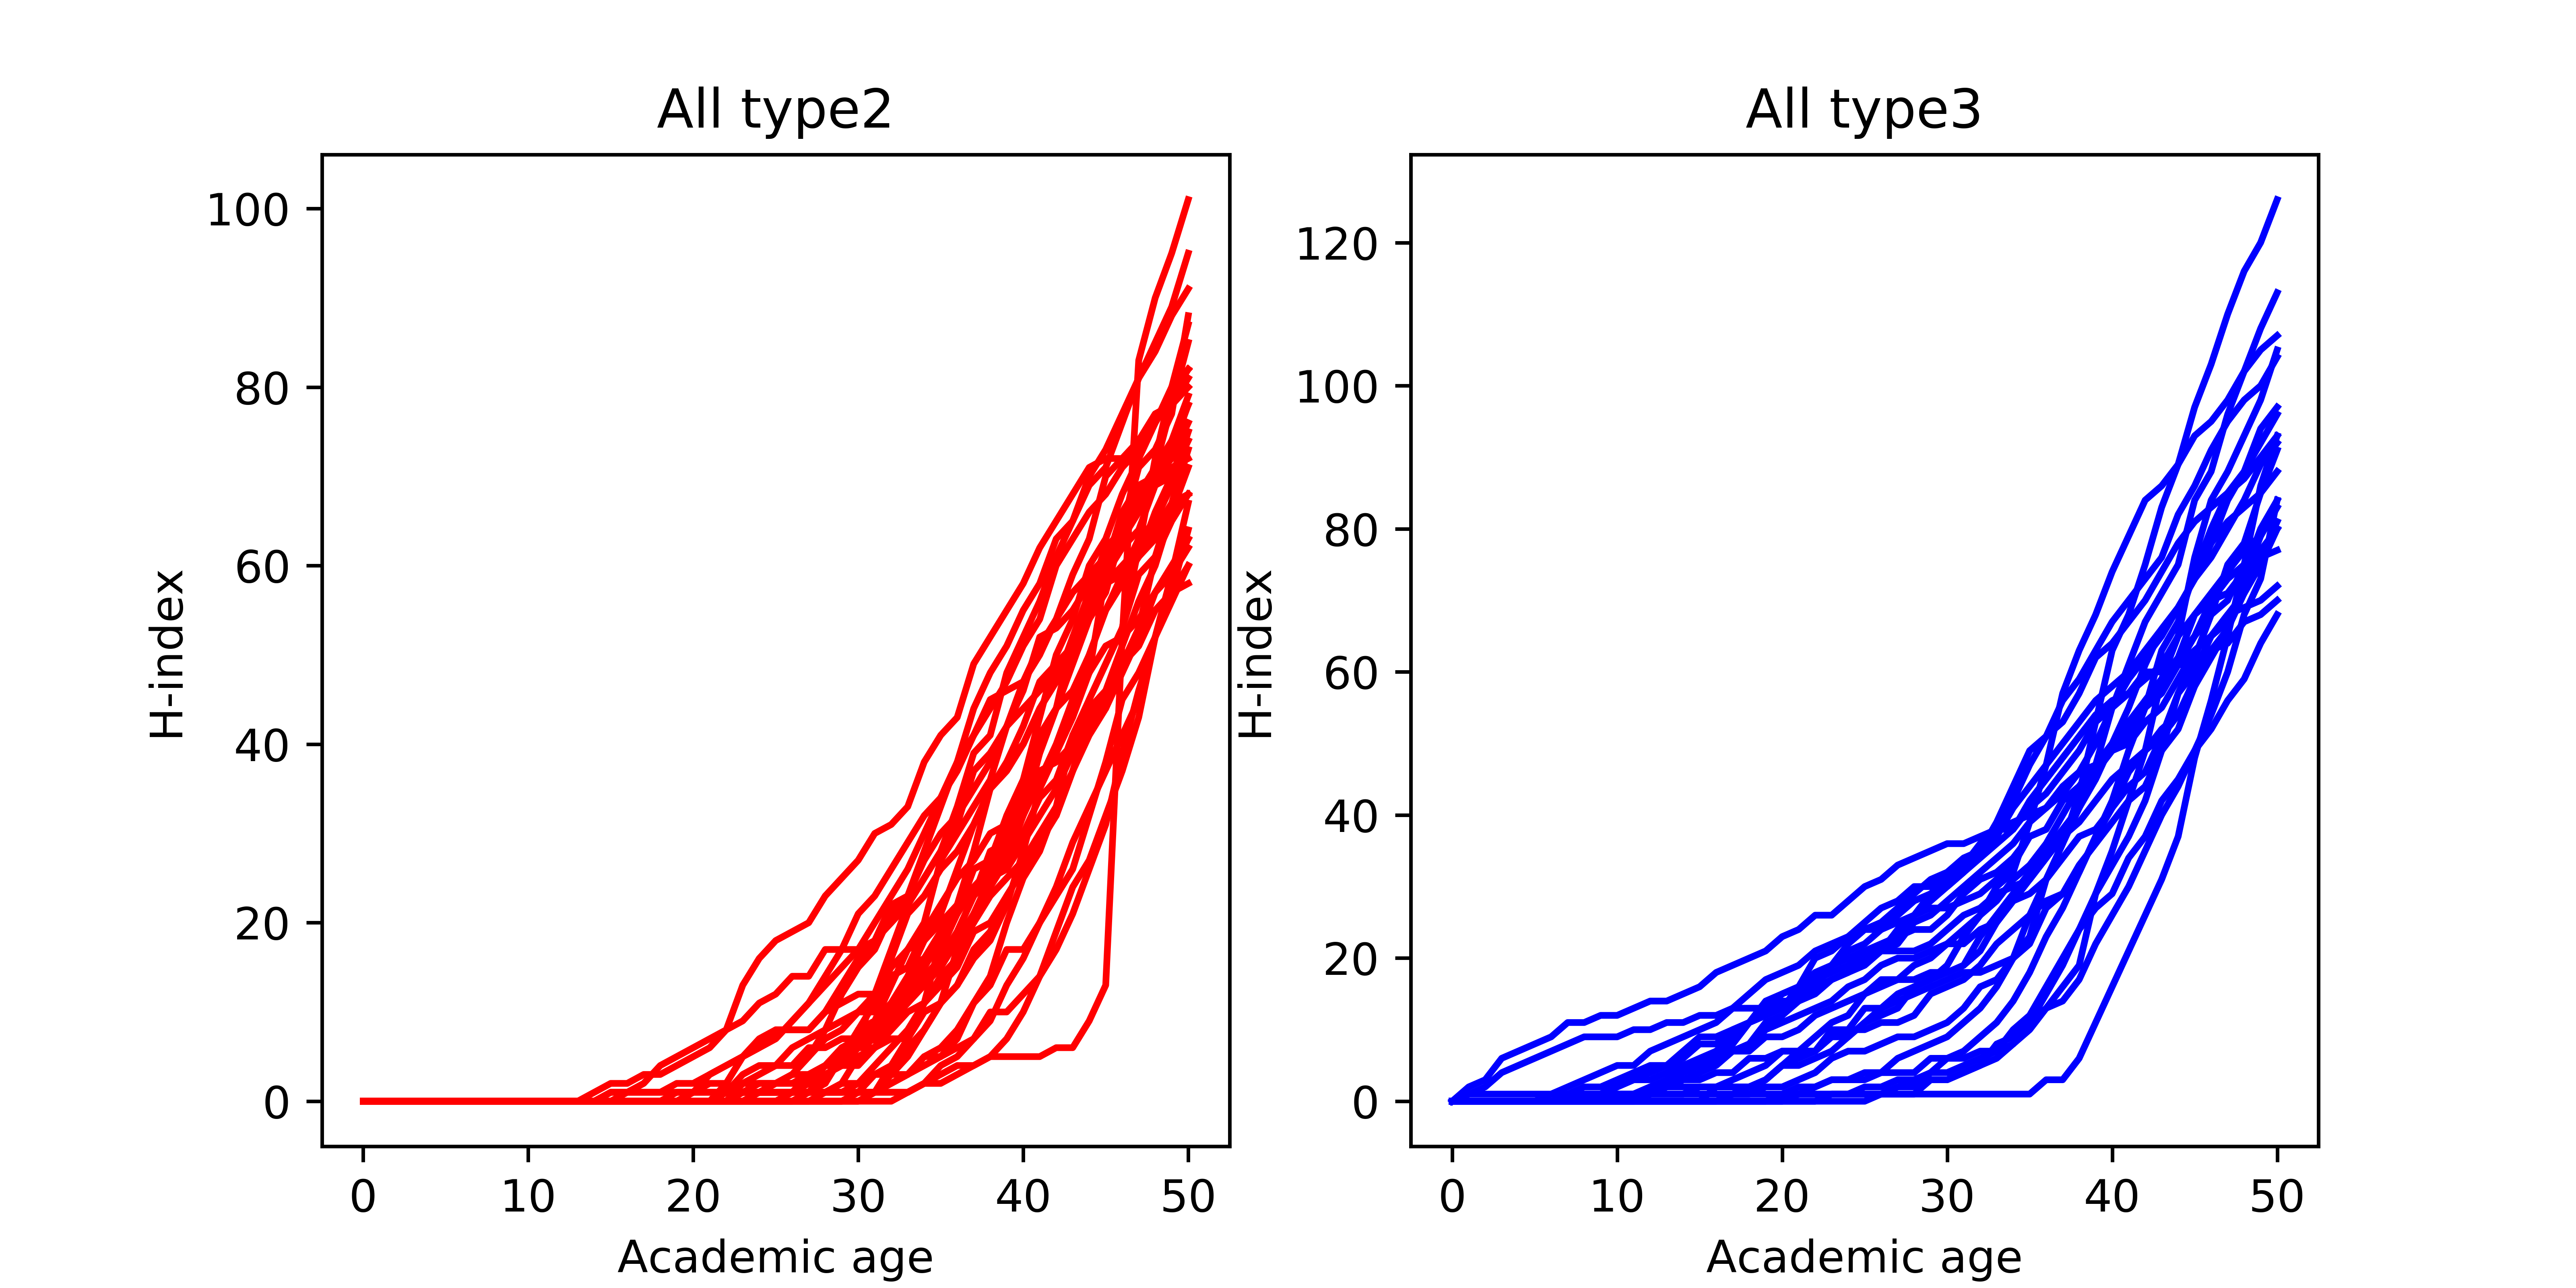
\includegraphics[width=0.9\textwidth]{image/type2_3.png}
	\caption{年轻型学者及文章量优势学者的H指数增长曲线}
	\label{fig5}
\end{figure}

本文数据集中学者的H指数普遍呈快速增长的指数模式,一个原因是这些学者都是学术影响力高的知名学者,H指数的增长即反映了他们极强的学术能力;我们认为另外一个可能的原因是数据集中的学者基本是计算机科学领域的学者,而计算机科学是近二三十年来发展最快的学科之一,学者们H指数的快速增长也许与整个研究领域的蓬勃发展密切相关。

\section{聚类启发式模型}

\subsection{模型构建}

在数据集分析部分我们通过观察分析聚类结果得到:较弱势学者的H指数增长近似\textbf{线性},而其他三类学者的H指数近似\textbf{指数}增长。受此启发,我们在得到需要预测的学者的信息后,可以先将其归类为四类学者中的一类,依据类别确定对应的增长模型,使用该学者的H指数历史数据拟合模型、确定模型参数,最后便可根据模型进行预测。我们将这一模型称为\textbf{聚类启发式模型},模型构建的具体步骤如下:

\begin{itemize}
	\item[1.] 模型所需数据:数据集分析部分里预先进行的聚类模型,所预测的学者从第一篇论文发表当年起的H指数历史数据、当前学术年龄、发表文章数量、总引用量。
	\item[2.] 将该学者当前的H指数值、学术年龄、发表文章数量、总引用量与聚类中心比较,选取与其中心的欧氏距离最近的类别,认为该学者为此类型学者。
	\item[3.] 根据该学者所属类别确定H指数增长模型。(较弱势学者对应线性模型,其他三类学者对应指数模型)
	\item[4.] 使用该学者H指数历史数据拟合增长模型,得到模型参数。
	\item[5.] 利用模型进行H指数值的预测。
\end{itemize}

其中步骤3中的线性模型和指数模型的表达式分别如下:
\begin{align*}
& \text{线性模型:} H_t = \beta_0 + \beta_1 t\\
& \text{指数模型:} H_t = \beta_0 + \alpha e^{\beta_1t}
\end{align*}

式中$t$表示学术年龄,$H_t$ 表示学术年龄为$t$时的H指数值,$\beta_0$、$\beta_1$和$\alpha$为需要估计的参数。值得说明的是,聚类启发式模型已考虑到对于不同年龄段学者H指数增长模式的不同,因为学术年龄已经作为一种聚类特征。实际上,该模型不仅仅包括学术年龄的影响,不是简单地将学者分为例如学术年龄20至30年、30至40年等阶段,再分别预测,而是采用更多维的数据,将学者分为具有实际意义的多种类别,依据所要预测的学者的所属类别进行更精细化的预测。

\subsection{预测实例}

我们选取清华大学姚期智教授的数据,依据模型构建部分所述的聚类启发式模型构建方法构建模型。姚期智教授截止2010年的相关数据如表(\ref{tab2})所示:

\begin{table}[H]
	\centering
	\caption{姚期智教授相关数据(截止2010年)}
	\label{tab2}
	\begin{tabular}{@{}llllll@{}}
		\toprule
		name & earliest\_year & h-index & co-author & paper\_num & citation\_num \\ \midrule
		Yao  & 1971           & 33      & 115       & 124        & 6610          \\ \bottomrule
	\end{tabular}
\end{table}

将其与预先聚类后得到的四个聚类中心进行比较,发现到较弱势学者群体的聚类中心的欧氏距离最短,于是将姚期智教授归类为较弱势学者。因为较弱势学者所对应的H指数增长模式为线性,故使用姚期智教授的历史H指数值拟合以下的线性模型:
$$H_t = \beta_0 + \beta_1 t$$

拟合出的参数如表(\ref{tab3})所示,其中$\hat{\beta}_1$在99\%的置信水平显著。

\begin{table}[H]
	\centering
	\caption{线性模型参数}
	\label{tab3}
	\begin{tabular}{@{}ccc@{}}
		\toprule
		$\beta_0$          & $\beta_1$            & $R^2$    \\ \midrule
		-1.1646(0.454) & $0.8969^{***}$(0.020) & 0.981 \\ \bottomrule
	\end{tabular}
\end{table}

将2011至2020年姚期智教授的H指数作为测试集,检验线性模型的预测效果,预测折线图如图(\ref{fig6})所示。其中预测的均方误差(\textit{Mean Square Error, MSE})为11.08。

\begin{figure}[H]
	\centering
	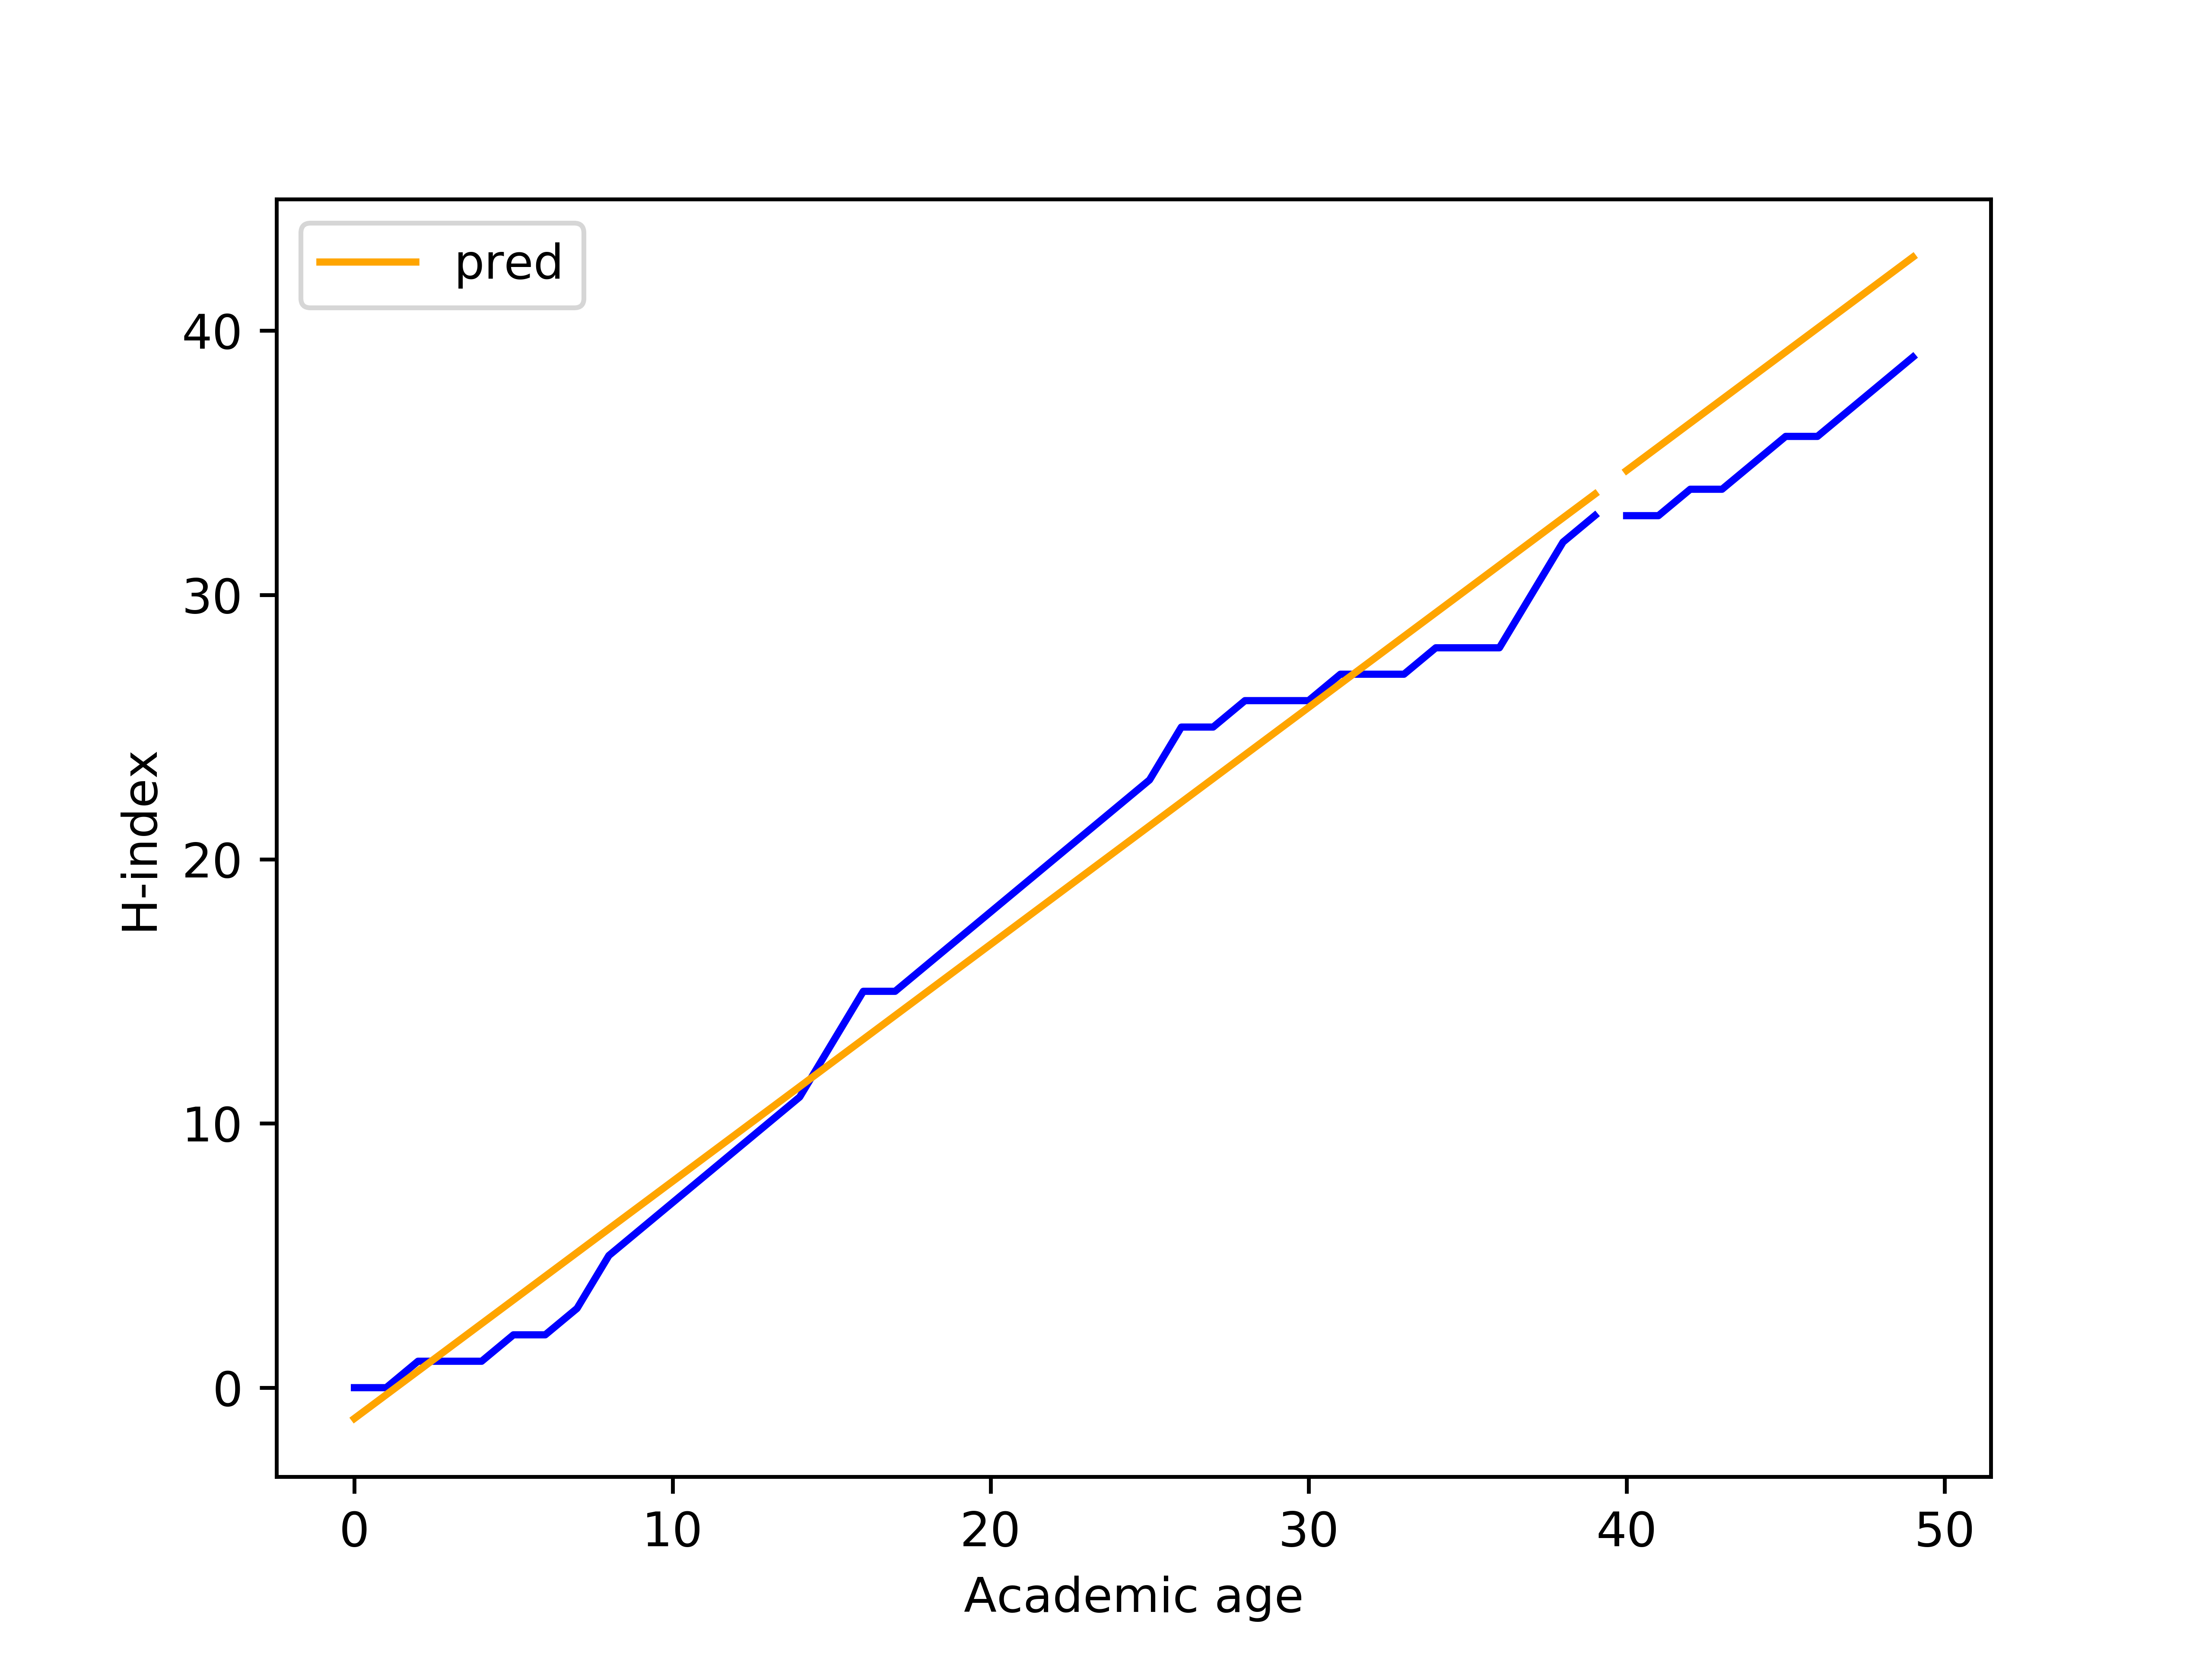
\includegraphics[width=0.6\textwidth]{image/yao.png}
	\caption{姚期智教授的H指数增长曲线及线性模型预测曲线}
	\label{fig6}
\end{figure}

观察图像我们发现姚期智教授的H指数增长曲线确实是呈近似线性,进而验证了聚类结果的可靠性。同时,线性模型能较好地拟合姚教授的H指数增长模式,虽然在预测时整体过于乐观,但把握住了变化的趋势,结果可以接受。

\subsection{模型评估}

虽然在上文的例子中聚类启发式模型有可接受的拟合与预测结果,但由于目前数据集中学者的数据较少,没有很好地发挥聚类分析提取额外信息的作用,且该模型有许多不可忽视的局限性:

\begin{itemize}
	\item[1.] 依赖于多种数据,若数据种类单一或有缺失值,对聚类的效果影响较大。
	\item[2.] 进行聚类的数据质量关系到模型的预测准确性。目前的数据集中数据量不足,聚类效果不是非常好,若有更多数量、种类的学者数据引入,能更好地区分不同类别学者的H指数增长模型,也能更准确地将所预测学者分入合适的类别,从而获得更好的预测结果。
	\item[3.] 只能进行短期预测。因为聚类的特征中包含了学术年龄,一些类别的模型仅对一定年龄段的学者有效。例如对于一个年轻型学者,使用对应的增长模型预测他未来5年的H指数值是合理的,但要想预测其20年之后的H指数则无法使用此方法,因为20年后该学者极有可能不再属于年轻型学者,而成长为其他类型的学者。
	\item[4.] 只能应用在同一或相似的学科领域。因为不同的学科之间学者的H指数值有较大的差距,导致聚类结果不准确。
	\item[5.] 目前的模型无法对学术年龄非常年轻的学者进行预测。因为当前聚类使用的数据集仅包括学术年龄18年以上的知名学者,要想使得模型推广至非常年轻的学者或非知名学者,就需要收集更多数量和类型的数据。
\end{itemize}

总之,聚类启发式模型的思想是充分利用学者自身的多种数据、其他学者的H指数增长模式等多维数据提供的信息精细化地确定增长模式。目前的模型有很大的改善空间,理论上用来进行预先聚类的数据集越丰富多样,模型的效果往往会更好。随着数据的增加,聚类所使用的类别数$k$也将随之增多,对更精细的类别进行描述解释,可能从中发现对该领域学者的学术影响力更深层的特点和启示,可作为未来对H指数预测研究的一个方向。

\section{ARIMA(p,d,q)模型}

根据\cite{PennerPan-511}的研究,学者的学术年龄对于预测他未来的H指数增长非常重要。于是我们将每个学者的H指数看成是一个时间序列,观察到未来的H指数与当前的H指数和过去的H指数有一定的关联,所以使用ARIMA模型进行预测有一定的合理性,而在这一部分中对实际数据的预测也表明使用ARIMA模型预测准确性较高。

\subsection{模型构建}

对于ARIMA(p,d,q)模型,我们首先要确定其最佳阶数。以AIC为准测,对每一条数据选取最佳的p, d, q,并将所有结果统计频数得到表(\ref{tab4})。

\begin{table}[H]
	\centering
	\caption{不同p, d, q出现频次}
	\label{tab4}
	\begin{tabular}{p{1cm}p{1cm}p{1cm}c}
		\hline
		p            & d            & q            & frequency \\ \hline
		0            & 2            & 0            & 7         \\
		0            & 2            & 1            & 42        \\
		0            & 2            & 2            & 6         \\
		1            & 2            & 0            & 15        \\
		1            & 2            & 1            & 2         \\
		1            & 2            & 2            & 3         \\
		2            & 2            & 0            & 4         \\
		2            & 2            & 1            & 1         \\
		2            & 2            & 2            & 9         \\ \hline
		\multicolumn{3}{c}{other parameter orders} & 7         \\ \hline
		\multicolumn{3}{c}{total}                  & 96        \\ \hline
	\end{tabular}
\end{table}

注意到有接近50\%的学者适用于ARIMA(0,2,1)模型,但这并不意味着对于其他学者而言,ARIMA(0,2,1)模型没有较好的拟合度,这是因为上述结果是以AIC为准则进行的参数选择。我们把每条数据使用ARIMA(0,2,1)模型以及使AIC最小的ARIMA模型$AIC_{opt}$分别进行数据拟合,得到的AIC数据对比如图(\ref{fig7})所示。

\begin{figure}[H]
	\centering
	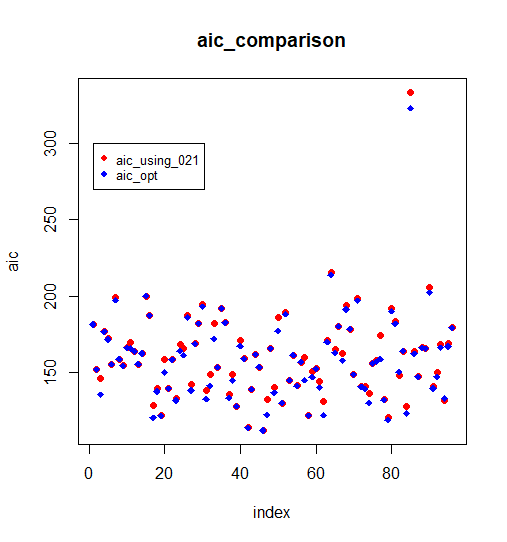
\includegraphics[width=0.6\textwidth]{image/aic.png}
	\caption{ARIMA(0,2,1)与最优ARIMA模型的AIC值对比}
	\label{fig7}
\end{figure}

图中红色数据点是使用ARIMA(0,2,1)模型拟合得到的AIC数值,而蓝色数据点是使用使得AIC最小的模型拟合得到的AIC数据。可以发现,对大部分数据点来说,模型ARIMA(0,2,1)与最优的ARIMA模型AIC数据相差不大,所以使用ARIMA(0,2,1)模型对于大部分数据来说是恰当的。我们随机抽取一名学者,分别画出H指数差分两次及其样本ACF、PACF如图(\ref{fig8})所示,均支持ARIMA(0,2,1)的模型假设。注意到第一幅图在前几年的H指数为0,表明该学者在前几年(从1970年开始)暂时未发表文章。而如果从第20年算起,则完全不影响时间序列平稳性以及模型的判断。

\begin{figure}[H]
	\centering
	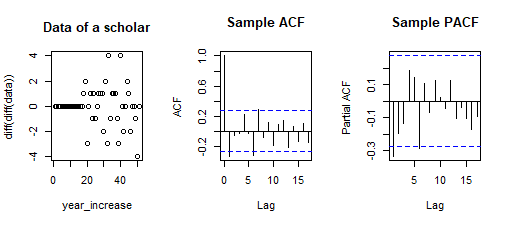
\includegraphics[width=0.9\textwidth]{image/sample_scholar.png}
	\caption{随机选取一名学者的时间序列分析}
	\label{fig8}
\end{figure}

\subsection{ARIMA(0,2,1)模型拟合与预测效果}

我们对于数据集中的所有数据,使用ARIMA(0,2,1)进行拟合,并计算模型残差的方差$\sigma^2$的估计值,画出图(\ref{fig9})。

\begin{figure}[H]
	\centering
	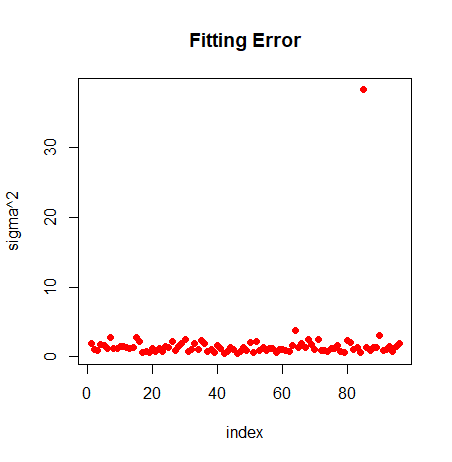
\includegraphics[width=0.6\textwidth]{image/sigma2.png}
	\caption{模型残差的方差的估计值}
	\label{fig9}
\end{figure}

除去离群值之后,得到模型的拟合误差处于较低水平,因此我们认为使用ARIMA(0,2,1)进行拟合的效果较好,其中,$\sigma^2$的估计值的平均值为1.358,方差为0.389。

对于数据集中的每一条数据,我们使用每一个学者前$i$年的数据作为已知数据,由此估计模型ARIMA(0,2,1)中的未知参数,并基于此模型对第$i+n$年的H指数值进行预测,计算预测误差的均值与方差作为评判依据。对于部分$i$与$n$的数值,预测的误差$\epsilon=H_{true}-H_{pred}$的均值与方差如表(\ref{tab5})与表(\ref{tab6})所示。

\begin{table}[H]
	\centering
	\caption{预测误差的均值}
	\label{tab5}
	\begin{tabular}{c|cccccccccc}
		$n$\textbackslash{}$i$ & 36     & 37     & 38     & 39     & 40     & 41     & 42     & 43     & 44     & 45     \\ \hline
		1                  & 0.5637 & 0.6073 & 0.0047 & 0.4508 & 0.126  & 0.4356 & 0.0412 & 0.0581 & 0.1726 & 0.4144 \\
		2                  & 1.4398 & 0.9125 & 0.4364 & 0.7869 & 0.5957 & 0.6733 & 0.1346 & 0.2724 & 0.6368 & 0.9226 \\
		3                  & 2.0139 & 1.6448 & 0.7536 & 1.4668 & 0.8675 & 0.9631 & 0.3841 & 0.7784 & 1.1947 & 1.1911 \\
		4                  & 3.0151 & 2.2625 & 1.4145 & 1.9488 & 1.1913 & 1.4091 & 0.9254 & 1.3782 & 1.5131 & 1.3451 \\
		5                  & 3.9016 & 3.2239 & 1.8776 & 2.4829 & 1.6715 & 2.1468 & 1.5603 & 1.7383 & 1.7169 & 1.3324
	\end{tabular}
\end{table}

\begin{table}[H]
	\centering
	\caption{预测误差的方差}
	\label{tab6}
	\begin{tabular}{c|cccccccccc}
		$n$\textbackslash{}$i$ & 36     & 37     & 38     & 39     & 40     & 41     & 42     & 43     & 44     & 45     \\ \hline
		1                  & 2.2576 & 1.8125 & 1.9591 & 3.1763 & 1.6137 & 1.9155 & 1.4862 & 2.4509 & 2.0032 & 3.2183 \\
		2                  & 6.1407 & 3.7774 & 6.7228 & 8.9908 & 4.737  & 5.0371 & 4.7586 & 6.3608 & 7.1244 & 25.021 \\
		3                  & 10.179 & 8.6098 & 15.388 & 17.016 & 8.7592 & 10.763 & 9.5659 & 13.091 & 35.449 & 67.909 \\
		4                  & 18.445 & 16.298 & 27.092 & 27.864 & 15.949 & 18.282 & 15.574 & 43.834 & 85.479 & 90.932 \\
		5                  & 30.142 & 25.74  & 43.691 & 46.913 & 24.859 & 26.258 & 48.36  & 95.252 & 112.86 & 113.09
	\end{tabular}
\end{table}

上述预测结果较好的反映了实际情况。随着$n$的增加,预测误差增加。我们发现预测误差的均值均为正值,这说明此模型有低估未来H指数的倾向。但即使如此,使用ARIMA(0,2,1)模型对H指数进行预测仍能在预测时间较小的范围内得到较为精确的预测值。

\subsection{预测实例}

为了进一步证明模型的有效性,我们选取清华大学姚期智教授的历史数据进行分析。姚期智教授的学术经验丰富,所以我们可以利用更多H指数的数据拟合模型。我们把前40年的数据代入模型中进行参数估计,并对之后10年的数据进行预测,结果如图(\ref{fig10})。可以发现预测值(蓝色数据点)与真实值十分接近。

\begin{figure}[H]
	\centering
	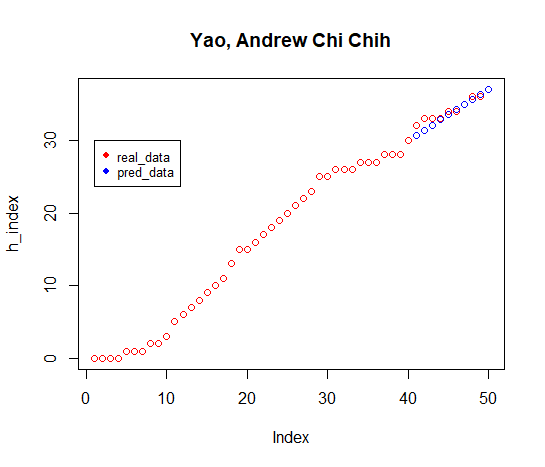
\includegraphics[width=0.6\textwidth]{image/yao_arima.png}
	\caption{姚期智教授H指数的ARIMA(0,2,1)模型预测}
	\label{fig10}
\end{figure}

事实上,ARIMA(0,2,1)模型对于相对资历教深的学者以及相对年轻的学者来说,预测效果都比较精确。所以对于不同年龄层次的学者,包括已经去世的学者,ARIMA(0,2,1)模型都有很强的适应性。只要提供一定量的数据,就能预测出较为准确的数值。但是,如果学者比较年轻,已知H指数数据较少,或学者成长速度过快,ARIMA(0,2,1)模型的预测就会产生一定的偏差。

清华大学的李国良是一位卓有成就且相对年轻的教授,我们使用他的数据,采用ARIMA(0,2,1)模型进行预测,结果如图(\ref{fig11})。可以看出该模型明显低估了学者H指数的增长,当然已知H指数数据较少是不可忽视的因素。经过对ARIMA(0,2,1)模型的进一步分析,我们发现,该模型预测时使用历史三年的数据的线性组合,对于“增长变快”的趋势,预测效果欠佳。

\begin{figure}[H]
	\centering
	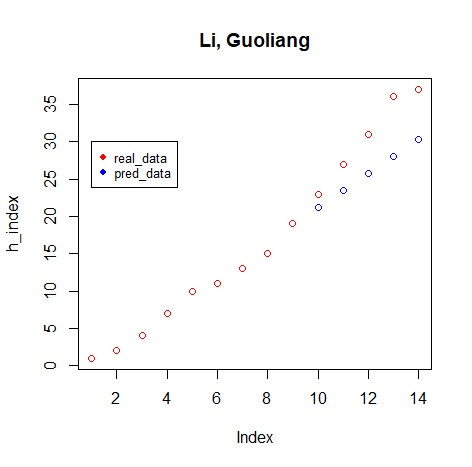
\includegraphics[width=0.6\textwidth]{image/lgl1.png}
	\caption{李国良教授H指数的ARIMA(0,2,1)模型预测(较长时间)}
	\label{fig11}
\end{figure}

但是,如果我们增加已知的H指数的值,并减少预测的年份,预测结果就会更加精确,如图(\ref{fig12})所示,此时对于未来两年的预测误差非常小,良好的完成了预测任务。

\begin{figure}[H]
	\centering
	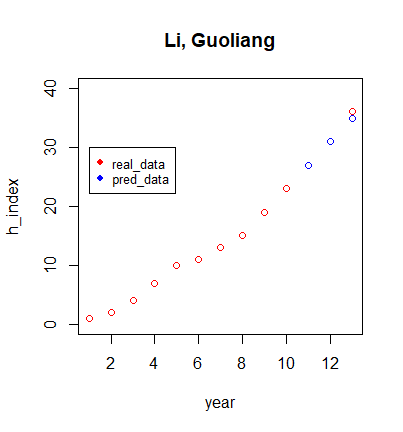
\includegraphics[width=0.6\textwidth]{image/lgl2.png}
	\caption{李国良教授H指数的ARIMA(0,2,1)模型预测(较短时间)}
	\label{fig12}
\end{figure}

\subsection{模型评估}

上述模型对于资深学者和领域专家来说,对于未来H指数的预测是较为准确的;但此模型对于年轻并且成长速度较快的学者来说,由于已知的有限数据只能体现出H指数较慢的增长速度,ARIMA(0,2,1)模型不能较好的预估出论文数量增长的趋势,从而对H指数增长的估计较为“保守”,其估计结果中H指数增长比真实情况偏慢,而随着预测时间的增长,预测误差也会逐渐累积。但总体而言,ARIMA(0,2,1)模型对于大部分层次的学者进行拟合和预测都非常稳健,不失为一种预测H指数的有效而精确的方法。

\section{总结与讨论}

\subsection{模型总结}

本文构建了基于聚类的预测模型和基于时间序列的ARIMA(0,2,1)两种预测模型。

基于聚类的预测受到\cite{7397965}的文章中多元回归预测的启发,将学术年龄、发表总文章数、总被引用量等数据作为聚类特征融入模型,提供分类别的、精细化的H指数增长模式确定方法。尽管聚类启发式模型在我们当前较小的数据集中表现得并不出色,筛选得到的不同类别的增长模式不够精细,但随着数据集大小的增加,聚类的结果将更加有意义,学者们H指数的增长规律也将逐渐明显,从而真正达到我们按类别特征进行精细化模型拟合、预测的目的。故聚类启发式模型应用在大数据集中效果将更好,由于我们无法得到如此大量的数据,便没有在大数据集中测试基于聚类的预测效果,如何更快速、准确地利用聚类方法进行大样本预测是未来研究的一个可能方向。

基于时间序列的预测则是根据已知的H指数的信息直接推断未来的信息,并没有直接使用学术年龄、发表总文章数等信息。ARIMA(0,2,1)模型的预测对于大部分学者都是非常精确的,而随着已知信息的增加,预测也更加精确。但是我们发现,当学者的H指数增长速度突然加快,甚至呈现指数增长的趋势的时候,在这一变化的临界点附近如果进行预测,则会产生较大的偏差。而事实上,任何模型都很难预测出学者在此临界点附近的表现。但我们可以根据获得的数据随时更新模型的参数,并更新未来的预测数据。ARIMA(0,2,1)模型在预测的准确性以及稳定性方面都具有较为优秀的表现,同时使用了更多历史H指数数据估计模型参数,并主要使用近几年的数据进行新数据的预测,从而预测准确性较高,而且适用于各个年龄段的学者。当然,对于在临界点附近的表现,我们可以通过加入其他信息进行判断,比如“此段时间学者发表文章数量突然增加”,或“发表一篇高质量且有影响力的文章,引文数量大幅增长”等信息来推断临界点是否发生,这是模型改进的方向,但这也要求我们获得更多的数据信息,需要对数据进行进一步的加工与处理。

\subsection{H指数合理性与有效性评价}

H指数已经是学界公认的评价学者学术影响力的较为有效的指标之一,且已经广泛使用多年,例如在Google Scholar中学者的个人界面,H指数与引用量、发表文章数等指标同时列出,其重要程度可见一斑。但H指数仍存在一些不合理之处,且已有许多学者尝试改进H指数,甚至提出新的评价指标。本文的重点并不是对H指数进行完善,所以接下来这部分将简要介绍H指数反映学者学术水平时的局限,并总结一些学者对于相应问题的解决方法。

\cite{Hirsch16569}在开篇提到,为了量化学者的科研成果,所以提出了H指数的指标,这可能用于大学教职员工的晋升、评奖等。因此,一个合理的H指数应当能够保证相对公平和正向激励。相对公平,成就越高的学者对应的H指数越高。正向激励,H指数应当避免使得学者通过“增加发表文章数量而不是质量”,“增加自引”而使H指数获得显著的提高。\cite{Hirsch16569}在结尾提到了以下几点问题:

\begin{itemize}
	\item 在非主流领域工作的学者,H指数可能相对偏低。即H指数高表明学者成就大,但学者成就大对应的H指数并不一定高。不同领域之间的H指数也可能存在较大的差异。
	\item 有些领域需要与更多的学者进行合作,所以一篇文章的作者可能有很多,这也使得一些学者的文章和引用数量因此得到大幅增加。我们应当考虑一篇文章的作者的数量。
	\item H指数与总引用数存在较强的函数关系,H指数并没有像它描述的那样合理。\cite{Alex}给出$h \approx 0.54 \sqrt{N_{citations}}$。
	\item 学者“科研年龄”的决定不应该是简单的发表第一篇文章,或者H指数不为0作为起始点,因为学者的前几篇文章可能仅做出次要贡献,并不能代表学者的水平。
	\item 应当删除学者“自引”的数据,因为自引可以显著增加H指数。
\end{itemize}

\subsection{H指数的改进}

上述问题有些可以通过数据收集而解决,例如依主要作者、第二作者的成就对引文数量进行加权计算;删除自引数据等。\cite{Egghe2006}提出了G指数的理论与实践。G指数是H指数的一种改进。一名学者的“G指数=$g$”表示,在他的所有论文中,引文数量最高的$g$篇论文的总引用数大于等于$g^2$,满足此条件的最大的$g$即为G指数。\cite{Egghe2006}证明了G指数的存在唯一性,并且G指数大于等于H指数。使用G指数则主要评估学者的主要学术成就,解决了部分学者通过增加发表文章数量和一定数量的文章引用(包括自引)等提高H指数的问题,同时对于非主流领域工作的学者成就的评估也相对更为客观。

\subsection{结论与展望}

对于本文的数据集,H指数是一个很好的评价学术影响力的指标。在对于数据集的分析中,我们发现H指数与学者的发表文章总数、被引用量有着很强的正相关关系,且在聚类时无论是引用量优势学者还是文章数优势学者,他们的H指数都是数据集中较高的水平。因而H指数的评价与直观的发表文章总数、被引用量一样,是较为客观合理的。有趣的是,不同于\cite{Hirsch16569}提到的H指数也许会更偏向于学术年龄长的学者,在本文的数据集中学术年龄在50年及以上的学者相对来说有着更低的H指数,一个可能的原因就是前文提到的领域相关问题,计算机科学领域在近些年会更加活跃,较为年轻的学者会比最资深的学者享有更多的发表和被引用机会;另外,数据选取也会有偏差,按照影响力高的知名学者这一标准来选取数据,在数据集中的各个学者几乎都是高水平的情况下,学术年龄越年轻,整体上就越能体现其水平高,H指数更高一些也不无道理。

总之,本文构建的需要数据量相对较少、较为简明的ARIMA模型在本文规模较小的数据集中有优秀的表现,同时还提出对数据集数量与质量要求较高的聚类启发式模型,在规模较大的数据集中能够获取更多信息,也是预测的有效方法。而H指数也能够较为合理有效地体现学者的学术影响力,所以本文的预测模型对于评估一个学者未来的影响力、研究成果有较大的意义。

\newpage
\nocite{*}
\bibliography{paper1}
%\bibliography{wpref}

%\appendix
%\appendixpage
%\addappheadtotoc



\end{document}
